\documentclass[11pt]{article}
\usepackage{amsmath}
%\usepackage{extsizes}
\usepackage{amsmath,amssymb}
%\usepackage{omegavn,ocmrvn}
%\usepackage[utf8x]{inputenc}
\usepackage[utf8]{vietnam}

\usepackage{longtable}
\usepackage{answers}
\usepackage{graphicx}
\usepackage{array}
\usepackage{pifont}
\usepackage{picinpar}
\usepackage{enumerate}
\usepackage[top=3.0cm, bottom=3.5cm, left=3.5cm, right=2.5cm] {geometry}
\usepackage{hyperref}


\usepackage{listings}
\lstset{language=Python}          % Set your language (you can change the language for each code-block optionally)


\newtheorem{bt}{Câu}
\newcommand{\RR}{\mathbb R}
\Newassociation{sol}{Solution}{ans}
\newtheorem{ex}{Câu}
\renewcommand{\solutionstyle}[1]{\textbf{ #1}.}
\newcommand{\m}[1]{
	\begin{bmatrix}
		#1
	\end{bmatrix}
}

\begin{document}
% \noindent
\begin{tabular*}
{\linewidth}{c>{\centering\hspace{0pt}} p{.7\textwidth}}
Trường ĐHKHTN, ĐHQGHN & {\bf Học Kỳ 1 (2020-2021)}
\tabularnewline
K63 TTƯD - MT\&KHTT \\ Lớp thầy Hà Phi & {\bf Bài kiểm tra giữa kỳ}
\tabularnewline
\rule{1in}{1pt}  \small  & \rule{2in}{1pt} %(Due date:)
\tabularnewline

%  \tabularnewline
%  &(Đề thi có 1 trang)
\end{tabular*}
%
% \Opensolutionfile{ans}[ans1]

\begin{center}	
\textbf{Đề III - Thi viết 60 phút}
\end{center}

\begin{bt}(4 $\times$ 1 = 4 điểm) \\
a)	Chứng minh rằng phương trình $7.5 + 6 x - x^3=0$ có nghiệm duy nhất trong đoạn $[2,3]$. \\
b)	Có rất nhiều các khác nhau để chuyển về bài toán tìm điểm bất động ($x=\varphi(x)$) để giải bằng phương pháp lặp đơn. Ta lấy ví dụ 2 phương pháp sau.
%
\[
i) \ \varphi(x) = \dfrac{x^3-7.5}{6} \ , \hskip 4cm \qquad  ii) \ \varphi(x) = \sqrt[3]{6x+7.5} \ .
\]
%
Hãy biện luận về tính hội tụ của các phương pháp trên. \\
Hai câu sau chỉ thực hiện cho phương pháp ii) . \\
c) Tìm số bước lặp cần thiết sao cho sai số tuyệt đối của nghiệm bé hơn $1e-9$, với $x_0 = 2.8$. \\
d) Tính $x_3$ chính xác đến 4 chữ số thập phân và đánh giá sai số hậu nghiệm cho $x_3$, với $x_0 = 2.8$. 
\end{bt}


\begin{bt}(4 $\times$ 1 = 4 điểm) \\
	a) Viết công thức lặp để giải hệ phương trình sau bằng phương pháp Jacobi. Phương pháp lặp này có hội tụ không? Vì sao?
	%
	\begin{align*}
	9 x_1 - 2 x_2 + 5 x_3 &= 1 \\
	1 x_1 + 7 x_2 + 1  x_3 &= 6 \\
	-1 x_1 - 3  x_2 + 7 x_3 &= -26 
	\end{align*}
	%
	b) Đối với hệ $x^{i+1} = M x^{i} + n$ mà các em vừa thu được bằng phương pháp Jacobi, hãy tìm $\|\cdot\|_1$ và $\|\cdot\|_{\infty}$ của ma trận hệ số $M$. \\
	c) Tính số bước lặp cần thiết bằng ước lượng tiên nghiệm sao cho ta có ước lượng sai số nghiệm $\|x^*-x^n\| \leq 1e-6$, với chuẩn $\|\cdot\|$ phù hợp và với $x^0$ tùy chọn. \\
	d) Cho $x^0 = \m{0 & 0 & 0}^T$. Hãy tìm $x^i$, $i=1,2,3$. Hãy sử dụng ước lượng hậu nghiệm để đánh giá sai số của $x_3$.
\end{bt}

\begin{bt}(2 điểm PLU + 2 điểm giải hệ) \\
Tìm phân tích PLU của ma trận 
\[
A = \m{1.78 & 2.34 & -4.10 \\
	   -2.22 & 1.98  & 3.47 \\
	  6.81 & 2.36  & -15.17}
\]
và hãy áp dụng để giải hệ sau
%
\[
A \m{x_1 \\ x_2 \\ x_3} = \m{0.02 \\ -0.73 \\ -6.63}
\]
%
\end{bt}
\cleardoublepage

\begin{center}	
	\textbf{ Đề II - Thi trên máy 60 phút}
\end{center}

\begin{bt}(3 điểm) \\ % Exercise 22, Kiusalass p.170 
	Thùng dầu hình trụ có bán kính r và chiều dài L được đổ đầy đến độ sâu h. Kết quả
	khối lượng dầu trong thùng là
	\[
	V = r^2L \Big( \phi - \left(1 - \dfrac{h}{r}\right) sin \phi \Big)
	\]
	trong đó $\phi = arcos\left(1 - \dfrac{h}{r}\right)$. Nếu bể đầy 3/4, hãy xác định tỉ số $h/r$.
	
	\begin{figure}[h!]
		\centering
		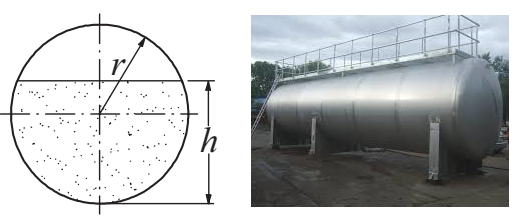
\includegraphics[width=0.7\linewidth]{oil_tank}
		\caption{}
		\label{fig:oiltank}
	\end{figure}
\end{bt}


\begin{bt}(3 điểm) \\
Cho một cơ cấu tay quay con trượt như trong hình dưới với AB = 0.5m, BC = 1m. Khâu dẫn 1 tạo với phương ngang 1 góc $\phi = $ 45 độ. Xác định vị trí của các khớp $B$, $C$ trong trường hợp này và góc tạo bởi khâu dẫn 2 và phương ngang. 
Hãy vẽ đồ thị hoành độ $x$ là hàm số thể hiện chuyển động của con trượt $C$ theo góc quay $\phi \in [0,360^o]$.
\begin{figure}[h!]
	\centering
	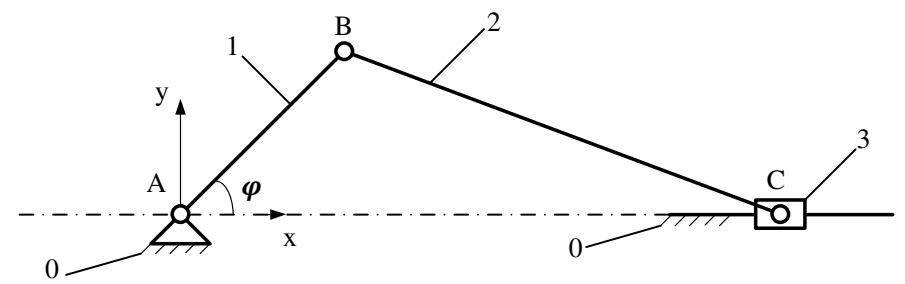
\includegraphics[width=0.7\linewidth]{tay_quay}
	\caption{}
	\label{fig:tayquay}
\end{figure}
\end{bt}

\begin{bt}(3 điểm) \\
Hãy vẽ đồ thị hàm số và lập trình phương pháp Newton để tính toán tất cả các nghiệm thực dương của phương trình
\[ 
f(x) = x^4 + 2x^3 - 7x^2 + 3 = 0,
\]
với sai số $1e-9$. So sánh với nghiệm (giả sử chính xác) có được bằng cách sử dụng hàm fsolve \verb|from scipy.optimize import fsolve| và tính sai số tương đối.
\end{bt}


\begin{bt}(3 điểm)
	Bốn vật nặng có khối lượng khác nhau $m_i$ được nối với nhau bằng những sợi dây có khối lượng không đáng kể. Ba trong số các khối nằm trên một mặt phẳng nghiêng, hệ số ma sát giữa các khối và mặt phẳng là $\mu_i$. Phương trình chuyển động của các khối có thể được biểu diễn là
	%
	\begin{align*}
		T_1 + m_1a &= m_1g (\sin \theta - \mu_1 \cos \theta) \\
		-T_1 + T_2 + m_2a &= m_2g (\sin \theta - \mu_2 \cos \theta) \\
		-T_2 + T_3 + m_3a &= m_3g (\sin \theta - \mu_3 \cos \theta) \\
		-T_3 + m_4a &= -m_4 g .
	\end{align*}
	%
	Trong đó $T_i$ biểu thị lực kéo trong các sợi dây và $a$ là gia tốc của
	hệ thống. Xác định $a$ và $T_i$ nếu $\theta = 45^o$, $g = 9,82 m / s^2$ và
	$m = \m{10 & 4 & 5 & 6}^T$ kg, $\mu = \m{0.25 & 0.3 & 0.2}^T$.
	%	
	\begin{figure}[h!]
		\centering
		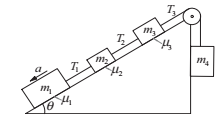
\includegraphics[width=0.4\linewidth]{mass_rope}
		\caption[]{Exercise 25, page 58, Kiusalass}
		\label{fig:massrope}
	\end{figure}
	
\end{bt}


\centerline{———————————Hết——————————-}

\vspace{1cm}
\noindent{\bf Chú ý:} {\it Cán bộ coi thi không giải thích gì thêm}\\

\cleardoublepage 


\begin{center}
	\textbf{ Bài tập lập trình.  \ Đề 1. Jacobi + Gauss-Seidel}
\end{center}

\begin{bt}
	Viết 2 hàm trong Python để giải hệ phương trình $Ax=b$ như sau
	%
	\begin{lstlisting}[frame=single] 
		def Jacobi(A,b,nmax,tol):
		return p
	\end{lstlisting}
	%
	và
	%
	\begin{lstlisting}[frame=single] 
		def Gauss_Seidel(A,b,nmax,tol):
		return p
	\end{lstlisting}
	%
	Ở đây nmax là số bước lặp tối đa, tol là sai số cần đạt được giữa nghiệm chính xác và nghiệm xấp xỉ.
	Trong script test luôn cho trường hợp $A =\m{-2 & 5 & 9 \\ 7 & 1 & 1 \\ -3 & 7 & -1}$, $b=\m{1 \\ 6 \\ -26}$ với nmax, tol tùy chọn.
\end{bt}

\begin{bt} % Che/Kincaid 07, page 503, Ex. 16
	Sử dụng hai hàm vừa viết trong bài trên để giải hệ phương trình sau với sai số $eps=1e-6$, $nmax=100$.
	\begin{equation*}
		\m{4 & -1 & 0 & 0 \\ -1 & 4 & -1 & 0 \\ 0 & -1 & 4 & -1 \\ 0 & 0 & -1 & 3} x = \m{15 \\ 10 \\ 10 \\ 10} \ .
	\end{equation*}
\end{bt}

%\end{document}

\vspace{1cm}
\noindent{\bf Chú ý:} {\it Cán bộ coi thi không giải thích gì thêm}\\
\Closesolutionfile{ans}
\newpage
\begin{center}
{\LARGE{\bf ĐÁP ÁN}}
\end{center}

\begin{sol}
Ta có thể xét các phép lặp đơn sau 
\begin{enumerate}
\item[i)] $\varphi(x) = 1+5x-10x^3$ (phân kỳ),
\item[ii)] $\varphi(x) = \cfrac{10x^3-1}{4}$ (phân kỳ),
\item[iii)] $\varphi(x) = \dfrac{1+4x}{10x^2}$ (hội tụ),
\item[iv)] $\varphi(x) = \sqrt{\dfrac{1+4x}{10x}}$ (hội tụ rất nhanh).
\end{enumerate}
%
The best solution would be iv), since the contraction constant on the interval $[0.7,0.8]$ is approximately $0.14$.
\end{sol}
   
\end{document}



